\documentclass[11pt]{article}
\usepackage[margin=1in]{geometry}
\usepackage[T1]{fontenc}
\usepackage{times,microtype}
\usepackage{amsmath,amssymb}
\usepackage{booktabs,graphicx,xcolor}
\usepackage[numbers,sort&compress]{natbib}
\usepackage[colorlinks=true,linkcolor=blue!60!black,citecolor=blue!60!black,urlcolor=blue!60!black]{hyperref}
\usepackage[capitalize,noabbrev]{cleveref}

\title{\textbf{The Body Connection Has Headroom That a Generic Learned Model Cannot Reach}}
\author{Manoj Bajaj \qquad Devin (Cognition AI)}
\date{}

\begin{document}
\maketitle

\begin{abstract}
A skill learned on one robot body can be reused on a related body by transporting each action through the two bodies' dynamics: predict the acceleration the source body would produce, then solve for the destination action that produces it. An earlier CPU pilot found that this state-dependent ``body connection'', learned with a generic random-feature dynamics model, lost to a six-parameter affine action map (EB12) on curved and contact-rich arm families. We ask whether the primitive lacks headroom or the estimator lacks data. With the true simulator in place of the learned model, the connection reaches 0.981 held-out return on the curved family against 0.925 for learned EB12 (+0.056, 4.3 standard errors over 16 paired seeds), and 0.962 against 0.839 on the contact family. The headroom is real. But the learned connection never beats EB12 at any ritual budget from 300 to 19{,}200 samples per body, including noise-free sensors, and on the curved family it gets worse between 4{,}800 and 19{,}200 samples. The shortfall is estimator bias, not variance. The preregistered estimator test fails; the connection stays parked until a structured dynamics model is available.
\end{abstract}

\begin{figure}[!h]
  \centering
  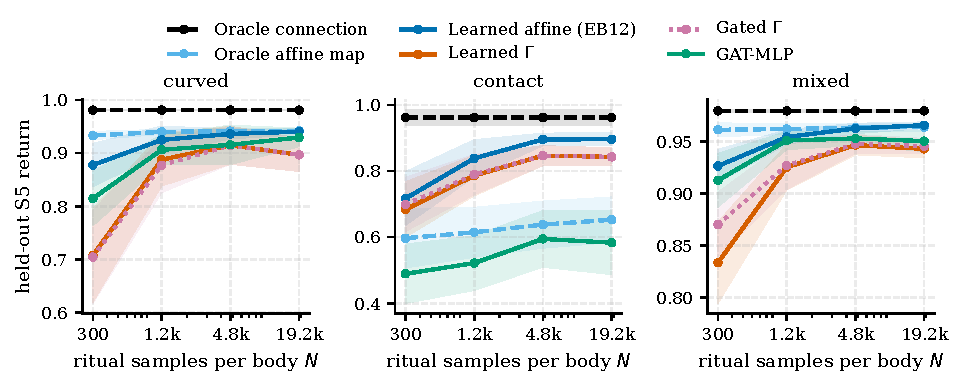
\includegraphics[width=\linewidth]{budget.pdf}
  \caption{\textbf{More ritual data does not let the learned connection reach the oracle.}
  Held-out return on the new skill S5 after transfer from the source body, against ritual samples per body, at 1\% sensor noise.
  Dashed lines use the true simulator: the exact connection (black) and the least-squares affine fit to it (light blue).
  Solid lines are learned from rituals. Bands are 95\% intervals over 16 seeds. GAT-MLP falls below 0.65 on contact.}
  \label{fig:budget}
\end{figure}

\section{Introduction}
\label{sec:intro}
A robot that keeps learning skills will eventually change bodies: a new link length, a heavier payload, a stiffer joint. Retraining every skill on the new body is wasteful when the bodies are related. Grounded action transformation~\citep{hanna2017gat} and learned inverse dynamics transfer~\citep{christiano2016transfer} reuse a source policy by mapping its actions through a model of both bodies. RMA~\citep{kumar2021rma} instead conditions one policy on a latent body estimate.

We studied a version of this idea that treats the transport as a learned connection \(\Gamma\) between bodies: a state-dependent map that sends a source action to the destination action producing the same acceleration. A CPU pilot in MuJoCo~\citep{todorov2012mujoco} fit \(\Gamma\) with generic random Fourier features~\citep{rahimi2007random} and promoted it only if it beat GAT-style and RMA-style controls with retention of at least 0.85. It failed 4 of 8 gates. With the same generic basis, \(\Gamma\) tied a GAT-MLP and lost to EB12, a six-parameter affine action map fitted to \(\Gamma\)'s own outputs.

That negative leaves two explanations open. Either the true transport between these bodies is close to affine, so no estimator of \(\Gamma\) can beat EB12, or the transport is far from affine and the learned model cannot recover it from 1{,}200 noisy rituals. These call for opposite next steps: drop the primitive, or invest in a better estimator. We preregistered a test that separates them by inserting the true simulator as an oracle and sweeping the ritual budget 64-fold and the sensor noise to zero.

The oracle connection beats EB12 by 0.03 to 0.25 held-out return on the curved and contact families at every budget and noise level (\cref{tab:main}), so the primitive has headroom. The learned connection does not approach it as data grows (\cref{fig:budget}). Its gap to EB12 stays negative at every budget and widens on the curved family, which points to bias in the generic model rather than to noise in its fit.

\section{Setup}
\label{sec:setup}
\paragraph{Bodies and skills.}
Each body is a two-link MuJoCo arm moving in a vertical plane under torque control. A family is a source body B and several related bodies. In the \emph{flat} family bodies differ only in actuator gains; in the \emph{curved} family they also differ in link masses, lengths and payload, so the inertia matrix changes with state differently on each body; the \emph{contact} family adds a unilateral wall whose position, compliance and friction vary by body; the \emph{mixed} family pairs B with three gain-only and three curved bodies. Each skill tracks a periodic joint trajectory. The new skill S5 is demonstrated only on B and must transfer to the other bodies of its family; we report its mean return over those held-out bodies. Return is \(\exp(-4\,\mathrm{MSE})\) of joint tracking over an 80-step horizon, averaged over 6 evaluation episodes. The flat family, where the pilot already found no gap, is not in the sweep.

\paragraph{Connection.}
Given control-affine dynamics \(\ddot q = B(q,\dot q)\,u + f(q,\dot q)\) for each body, the connection maps a source action \(u\) at state \((q,\dot q)\) to the least-squares destination action
\begin{equation}
  \Gamma(q,\dot q)\,u = \arg\min_{u'} \big\| B_{\mathrm B}u' + f_{\mathrm B} - (B_{\mathrm A}u + f_{\mathrm A})\big\|^2 .
  \label{eq:gamma}
\end{equation}
The learned connection fits \(B\) and \(f\) for each body by ridge regression on random Fourier features of \(q\) and \((q,\dot q)\), using \(N\) ritual samples of random states and actions per body. The oracle connection replaces the learned forward and inverse models with MuJoCo's own forward dynamics on A and inverse dynamics on B, evaluated at the observed state.

\paragraph{Arms.}
All arms see the same rituals, skill data and seeds. \textbf{EB12} fits an affine map \(u\mapsto Mu+c\) (six parameters for two joints) by least squares to the learned \(\Gamma\)'s outputs on ritual states. \textbf{Oracle affine} fits the same affine map to the oracle connection's outputs; it is the best affine approximation of the true transport over the ritual distribution. \textbf{Gated \(\Gamma\)} uses the ED08 split-half curvature statistic from the pilot to choose between learned \(\Gamma\) and EB12 for each family. \textbf{GAT-MLP} learns forward and inverse MLPs~\citep{hanna2017gat,christiano2016transfer}. \textbf{No transport} applies A's actions unchanged. For retention, demonstrations of the old skills S1--S4 from every body are pooled on B through each arm's transport, fit as one policy per skill, and sent back to every body; retention is the mean return.

\paragraph{Preregistered bar.}
Before running the sweep we fixed three tests, each on held-out S5 return with paired differences over 16 seeds:
\textbf{K1 headroom}: on the curved family at \(N=1{,}200\) and 1\% noise, the oracle connection beats learned EB12 by more than 2 SE and by at least 0.010.
\textbf{K2 estimator}: at some budget \(N\in\{300,1200,4800,19200\}\) at 1\% noise, gated \(\Gamma\) beats both EB12 and GAT-MLP by more than 2 SE on both curved and contact.
\textbf{K3 retention}: at that budget, gated \(\Gamma\)'s retention is at least 0.85 on curved and contact.
K1 failing would retire the primitive. K1 passing with K2 failing would retire this estimator. We also predicted that if the shortfall were estimator variance, the learned \(\Gamma\)--EB12 gap would shrink monotonically with \(N\) and close at zero noise.

\section{Results}
\label{sec:results}
\paragraph{The harness reproduces the pilot.}
Rerunning the original pilot with MuJoCo 3.17.0 reproduces every reported number and the \textsc{no-promote} verdict bit for bit.

\begin{table}[t]
  \centering
  \caption{\textbf{The oracle connection beats every affine map; the learned connection loses to EB12.}
  Held-out S5 return on the non-source bodies at 1\% sensor noise, mean \(\pm\) 95\% interval over 16 seeds. \(N=1{,}200\) is the pilot's budget.
  Oracle rows use the true simulator and are upper references, not deployable arms.}
  \label{tab:main}
  \footnotesize
  \setlength{\tabcolsep}{2.5pt}
  \begin{tabular}{lcccccc}
    \toprule
    & \multicolumn{3}{c}{\(N=1{,}200\)} & \multicolumn{3}{c}{\(N=19{,}200\)} \\
    \cmidrule(lr){2-4}\cmidrule(lr){5-7}
    Arm & curved & contact & mixed & curved & contact & mixed \\
    \midrule
    \csname @@input\endcsname table_main.tex
    \bottomrule
  \end{tabular}
\end{table}

\paragraph{K1 passes: the true transport is not affine.}
On the curved family at the pilot's budget, the oracle connection scores 0.981 against 0.925 for learned EB12, a paired gain of 0.056 at 4.3 SE (\cref{tab:main}). The gain grows to 14.5 SE at \(N=19{,}200\) because EB12's own variance shrinks. On contact the oracle scores 0.962, and the gap to EB12 is 0.12 at \(N=1{,}200\) and 0.07 at \(N=19{,}200\). The oracle matches the inverse-dynamics expert (0.98 on every family). Its affine projection loses most of the headroom: 0.940 on curved, and only 0.61--0.65 on contact, below learned EB12. We suspect this is because the least-squares fit is weighted by random ritual states, many of them in contact, while the S5 trajectories spend little time against the wall; the learned \(\Gamma\) is smoother and its affine fit happens to suit S5 better. Either way, no affine map in this harness comes close to the oracle on contact.

\begin{table}[t]
  \centering
  \caption{\textbf{The learned connection's gap to EB12 never turns positive.}
  Paired difference in held-out S5 return, mean (gap in SE), over 16 seeds; ``ret.'' is gated \(\Gamma\)'s S1--S4 retention. K2 needs the middle column of each family to be above \(+2\) SE together with the gated \(\Gamma\)--GAT column.}
  \label{tab:sweep}
  \small
  \setlength{\tabcolsep}{3pt}
  \begin{tabular}{rccccccccc}
    \toprule
    & & \multicolumn{4}{c}{curved} & \multicolumn{4}{c}{contact} \\
    \cmidrule(lr){3-6}\cmidrule(lr){7-10}
    \(N\) & noise & oracle\(-\)EB12 & \(\Gamma-\)EB12 & gated\(-\)GAT & ret. & oracle\(-\)EB12 & \(\Gamma-\)EB12 & gated\(-\)GAT & ret. \\
    \midrule
    \csname @@input\endcsname table_sweep.tex
    \bottomrule
  \end{tabular}
\end{table}

\paragraph{K2 fails at every budget.}
The learned connection is below EB12 at every budget and both noise levels on curved, contact and mixed (\cref{tab:sweep}). On curved it rises from 0.707 at \(N=300\) to 0.915 at \(N=4{,}800\), then falls to 0.897 at \(N=19{,}200\), while EB12 rises steadily to 0.940. Gated \(\Gamma\) beats GAT-MLP by a wide margin on contact, where GAT-MLP stays below 0.60 at 1\% noise, but never on curved. Because K2 requires both families, no budget qualifies.

\paragraph{The shortfall is bias, not variance.}
Both preregistered variance predictions fail. The gap does not shrink monotonically with \(N\): on curved it is \(-0.037\) at 1{,}200, \(-0.021\) at 4{,}800 and \(-0.044\) at 19{,}200. Removing sensor noise lifts every arm but leaves the learned connection below EB12 (\(-1.8\) SE on curved and \(-3.3\) SE on contact at \(N=1{,}200\)). A model whose error came mainly from too few or too noisy samples would close the gap in one of these conditions. We hypothesize that the generic feature basis cannot represent the state-dependent inertia and contact terms that the transport depends on, and that its fixed ridge penalty biases \(B\) toward a smooth average. We did not test alternative bases or penalties.

\paragraph{K3 fails on contact.}
Gated \(\Gamma\)'s retention on curved reaches 0.94--0.96 at large budgets but stays at 0.39--0.67 on contact at every budget and noise level. The oracle connection retains 0.90 on contact at 1\% noise and 0.98 without noise, so the failure is again in the estimate, not the primitive.

\section{Related work}
\label{sec:related}
Grounded action transformation learns a forward model of the target and an inverse model of the source to correct simulator actions~\citep{hanna2017gat}; \citet{christiano2016transfer} map simulated next states to real actions through a learned inverse dynamics model. Both are instances of \cref{eq:gamma} with neural estimators, which our GAT-MLP arm represents. RMA conditions one policy on a latent estimate of the body~\citep{kumar2021rma}; the pilot found a capacity-matched RMA closed most of the original gap. Our contribution is not a new transfer method but an oracle decomposition of a failed one: it shows that the state-dependent transport is worth 0.03 to 0.25 return over the learned affine map in this harness, and that a generic random-feature estimator~\citep{rahimi2007random} recovers none of it.

\section{Conclusion}
\label{sec:conclusion}
State-dependent action transport between related arms has real headroom over an affine action map in MuJoCo, especially with contact. A generic learned connection does not reach it with up to 19{,}200 ritual samples per body or with noise-free sensors, so the earlier negative was an estimator failure, not a primitive failure. The preregistered estimator test fails and the idea stays parked. The next test worth running replaces random features with a structured rigid-body model whose inertia and contact terms are identified from rituals, and keeps the oracle arm as a ceiling. This study covers two-link planar arms, one skill family and one random-feature basis; other bodies and estimators may behave differently. Code, preregistration and seed-level results are in the \href{https://github.com/manojbajaj95/cl/tree/main/experiments/body_connection}{code repository}.

\paragraph{AI disclosure.}
Manoj Bajaj and Devin (Cognition AI) jointly selected this idea from the project's research ledger; Manoj Bajaj set the research direction. Devin designed and preregistered the oracle and budget test, verified the cited literature records, implemented and ran the experiments, analyzed the results, and wrote the paper. Idea selection was mixed; literature, experiments, analysis and writing were done by Devin.

\bibliographystyle{plainnat}
\bibliography{references}

\end{document}
